%
\documentclass{gmto}

% - - - - - - - - - - - - - - - - Some extra packages - - - - - - - - - - - - - - - -
\usepackage[load=accepted]{siunitx}
\usepackage{subcaption}
\usepackage{amsmath, amssymb}
\usepackage{todonotes}
\usepackage{dirtytalk}
\usepackage{biblatex}
\usepackage{tikz}
\newcommand*\circled[1]{\tikz[baseline=(char.base)]{
            \node[shape=circle,draw,inner sep=0.4pt] (char) {\color{red}{\small #1}};}}

% - - - - - - - - - - - - - - - -
%\addbibresource{m1.bib}
\addbibresource{gmto.bib} % Use biber


% - - - - - - - - - - - - - - - -
\newcommand{\argmin}[1]{\underset{#1}{\operatorname{arg}\,\operatorname{min}}\;}
% lower-case letters (to represent actuator locations)
\DeclareFontFamily{U}{mathc}{}
\DeclareFontShape{U}{mathc}{m}{it}{<->s*[1.03] mathc10}{}
\DeclareMathAlphabet{\mathscr}{U}{mathc}{m}{it}
\def \actCoord#1#2 {\mathscr{#1}_{#2}}

% - - - - - - - - - - - - - - - -
\DocID{GMT-DOC-XXXXX}
\DocVersion{1.0}
\DocStatus{Draft}

%\title{Polishing error mitigation: a bi--objective optimization approach to compute the compensation forces}
\title{Polishing error mitigation}
\subtitle{A two--objective optimization approach to compute compensation forces}
% Though the term bi-objective is often used, it was replaced with two-objective
\author{R.~Romano, R.~Conan, and C.~Dribusch}
\date{\today}

%\tolerance=1000
%\hyphenpenalty=1000.

\begin{document}

\maketitle

\clearpage

\section*{Signatures}
\vspace{1cm}
\subsection*{Author}
\vspace{1.5cm}
%\tabulinesep=1em
\begin{tabu} to \linewidth {X[3,l]X[1,l]}
  \rule{\linewidth}{.1pt} & \rule{\linewidth}{.1pt} \\
  Name, title & Date
\end{tabu}
\vspace{1.5cm}
\subsection*{Approvers}
\vspace{1.5cm}
%\tabulinesep=1em
\begin{tabu} to \linewidth {X[3,l]X[1,l]}
  \rule{\linewidth}{.1pt} & \rule{\linewidth}{.1pt} \\
  Name, title & Date \\[1cm]
  \rule{\linewidth}{.1pt} & \rule{\linewidth}{.1pt} \\
  Name, title & Date
\end{tabu}

\clearpage

\section*{Revision Log}

\begin{revisions}
  1.0 & \today & All & None & Initial version & Author \\  
\end{revisions}

\clearpage

\tableofcontents
\listoffigures
\listoftables

\clearpage

\section{Purpose}
\label{sec:purpose}

This document describes an optimization approach to compute polishing error compensation forces. The strategy is based on a two--objective cost function. One is the residual surface error, and the other is linked to the tension induced by compensation. Our goal is to show that it can be advantageous to use the proposed method to compensate for mirror shape error characterized a priori.



\section{Introduction}
\label{sec:introduction}

The primary mirror active support incorporates pneumatic force actuators to hold the mirror and to control its surface. This task is accomplished by applying a controlled force vector to the back surface of the mirrors through pucks that are bonded to the mirror back surface. These support actuators are also used to correct for mirror deformations that are created by the effect of gravity, wind and thermal disturbances.

An outer ring of single--axis actuators and another set of triple--axis ones composes the actuator array. %%Figure~\ref{fig:supportActuators} illustrates the layout of single and triple--axis support actuators.
The first type applies forces in the normal direction to the back surface of the mirror, while triple--axis actuators can apply forces in $3$ directions. There are $80$ single and $85$ triple actuators for the outer segments (a total of $n_a=165$ actuators with $n_u = 335$ degrees of freedom) and $n_a=154$ actuators for the center segment, providing $n_u = 306$ degrees of freedom through $78$ single and $76$ triple actuators.


The fabrication shape error of M1 is one of the most significant contributors to the image quality error. The current best estimate (CBE) assumes the residual shape error after the correction obtained with the linear combination of the right singular vectors relative to the first $27$ bending modes \cite[Section 6.3.1.1]{GMT_DOC_04680}. That method is hereafter referred to as the baseline. The resulting PSSN is $0.9566$ and $0.9895$ at \SI{0.5}{\micron} and \SI{1.65}{\micron}, respectively. A full description of the simulations can be found in \cite{GMT_DOC_04637}.

This technical note proposes a two--objective optimization approach to compute polishing error compensation forces. Simulation results indicate that the open--loop compensation using those forces can significantly improve the image quality for the Natural Seeing (NS) observation mode. The results also indicates that the mirror tension induced by those forces is lower that observed with the baseline correction.%
It should be stressed that the algorithm described here to cope with the polishing error is a particular case of a method originally developed to compute the gravity support forces (refer to \cite{Romano2020a}).


%This report presents a least--squares optimization (LSO) approach to compute the support actuator forces. Section~\ref{sec:ls_FdistAlg} describes the force balance algorithm. Section~\ref{sec:simResults} shows the performance of the proposed approach from the simulation of gravity load on different zenith angles. Results in case of actuator failures are also discussed. Concluding remarks are drawn in Section~\ref{sec:conclusions}.



\section{Computation of the polishing error compensation forces}
\label{sec:opt_method}

We assume the use of support actuator offset forces $u \in \mathbb{R}^{n_u}$ to compensate for the polishing error in open--loop. Our goal is to develop an algorithm that computes $u$, managing two conflicting goals. The first is to minimize the shape error, and consequently, the wavefront error caused by each mirror segment. The second is to come up with a set of forces that leads to admissible mirror glass stress. On top of that, the obtained solution should not result in net forces and moments on the mirror. 

Consider the matrix $M_r \in \mathbb{R}^{n_u \times 3n_a}$ filled with $0$s and $1$ to remove lateral and cross--lateral force entries corresponding to single actuators, such that
\begin{equation} \label{eq:alternative_u}
u = M_r
\begin{bmatrix}
f_{x_1} & f_{y_1} & f_{z_1} & \cdots & 
f_{x_{n_a}} & f_{y_{n_a}} & f_{z_{n_a}}
\end{bmatrix}^T,    
\end{equation}
where the notation $f_{x_k}$ indicates the force applied along $\vec{x}$ by actuator $k \in \{1,\ldots,n_a\}$. Let $s_{\text{p}}$ an $n_s$--dimensional vector representing the fabrication surface error. We represent the compensated residual surface shape error as 
%
\begin{equation}
\label{eq:surf_error}
s_\epsilon = s_{\text{p}} - A_f M_r^\dagger u,
\end{equation}
where $M_r^\dagger$ denotes the left--inverse of $M_r$ and $A_f \in \mathbb{R}^{n_s \times 3n_a}$ combines the columns of the lateral, cross--lateral, and axial influence matrices, each mapping the support actuator forces vectors along an orthogonal axis of the segment coordinate system ($\vec{x}$, $\vec{y}$, and $\vec{z}$, respectively) into mirror surface nodes axial displacements. The computation of the influence matrices from the finite--element model (FEM) of the mirror is approached in \cite[Section 3]{m1SupportF2017}. For outer--axis segments, the mirror FEM has $n_s = 27685$ surface nodes (rows in the influence matrices). The center segment influence matrices have $n_s = 25794$ rows.



%\subsection{Polishing error compensation problem formulation}


To accommodate the conflicting goals for the compensation forces, it is proposed the quadratic cost function
\begin{equation}
\label{eq:J}
J = \rho\left\| s_\epsilon \right\|_2^2 + \|W u\|_2^2 
\end{equation}
where the notation $\left\| \cdot \right\|_2$ represents the Euclidean norm, i.e.
\[
\left\| s_\epsilon \right\|_2^2 = s_\epsilon^T s_\epsilon .
\]
The positive constant $\rho$ adjusts the trade--off between the residual shape error and the magnitude of the compensation forces. The weighting matrix $W$ is strictly diagonal, whose main diagonal elements $w_{ii}$ assume values according to the number of pucks $n_p$ of each actuator\footnote{The primary mirror support design considers actuators with 1 to 4 pucks.}, that is, $w_{ii} = 1/\sqrt{n_p}_i$, for $i \in \{1, \ldots, n_u\}$.

From \eqref{eq:alternative_u}, the matrix $\Upsilon \in \mathbb{R}^{6 \times n_u}$ that maps the support actuator forces $u$ into the vector $\tau$ of net forces and moments on the mirror reads as
\[
\Upsilon = 
\begin{bmatrix}
1 & \cdots & 1 & 0 & \cdots & 0 & 0 & \cdots & 0 \\
0 & \cdots & 0 & 1 & \cdots & 1 & 0 & \cdots & 0 \\
0 & \cdots & 0 & 0 & \cdots & 0 & 1 & \cdots & 1 \\
0 & \cdots & 0 & -\actCoord{z}{1} & \cdots & -\actCoord{z}{n_a} %
& \actCoord{y}{1} & \cdots & \actCoord{y}{n_a} \\
\actCoord{z}{1} & \cdots & \actCoord{z}{n_a} & 0 & \cdots & 0 %
& -\actCoord{x}{1} & \cdots & -\actCoord{x}{n_a} \\
-\actCoord{y}{1} & \cdots & -\actCoord{y}{n_a} %
& \actCoord{x}{1} & \cdots & \actCoord{x}{n_a} %
& 0 & \cdots & 0
\end{bmatrix}
M_r^{\dagger} ,
\]
%
where $\left[\actCoord{x}{k} \ \actCoord{y}{k} \ \actCoord{z}{k} \right]^T$ is the $k$th support actuator geometric coordinate vector with respect to the center of gravity (CG) of the mirror. %
%The set of forces and moments about axes $\vec{x}$, $\vec{y}$, and $\vec{z}$ composes $\tau$, namely
%\[
%\tau =
%\begin{bmatrix}
%    \tau_{f_x} & \tau_{f_y} & \tau_{f_z} &
%    \tau_{m_x} & \tau_{m_y} & \tau_{m_z}
%\end{bmatrix}^T .
%\]
%
Therefore, from \eqref{eq:surf_error} and \eqref{eq:J}, the vector of optimized compensation forces $u^\ast$ is given by
\begin{equation} \label{eq:LSOproblem}
u^\ast = \argmin{u} \frac{\rho}{2}\left\| s_{\text{p}} + A_f M_r^\dagger u \right\|_2^2 + \frac{1}{2}\|W u\|_2^2   ,
\end{equation}
subject to $\Upsilon u = \begin{bmatrix}
0 & 0 & \cdots & 0
\end{bmatrix}^T$.

As shown in Appendix~\ref{sec:OPT_sol}, the optimization problem \eqref{eq:LSOproblem} has the analytical solution
\begin{equation}
\label{eq:LSOsol}
u^\ast = 
\begin{bmatrix}
I_{n_u} & \mathbf{0}_{n_u \times 6}
\end{bmatrix}
\begin{bmatrix}
\rho \Lambda^T\Lambda + W^TW & \Upsilon^T \\ \Upsilon & \mathbf{0}_{6 \times 6}
\end{bmatrix}^{-1} \begin{bmatrix}
- \rho \Lambda^T s_{\text{p}} \\ \mathbf{0}_{6 \times 1}
\end{bmatrix},
\end{equation}
where $I_{n_u}$ is an $n_u$--dimensional identity matrix, the notation $\mathbf{0}_{n_1 \times n_2} \in \mathbb{R}^{n_1 \times n_2}$ represents zero matrices, and $\Lambda = A_f M_r^\dagger$.


\section{Simulation Results}
\label{sec:simulations}

The Richard F. Caris Mirror Lab provided the surface error of segments \textsf{S1} and \textsf{S2}, with the mirrors pointed to the zenith. For this study, the original surface maps were resampled to match the node locations of the mirror FEM mesh using a linear interpolation algorithm. The vector $s_{\text{p}}$ is a stacked version of the resampled surface error maps. As the polishing error profile is available just for \textsf{S1} and \textsf{S2}, we assume the latter for the center segment (\textsf{S7}). Figure~\ref{fig:pol_error_maps} depicts the polishing error maps considered in this study.
%
\begin{figure}[!hbt]
    \vspace{6pt}
    \centering
    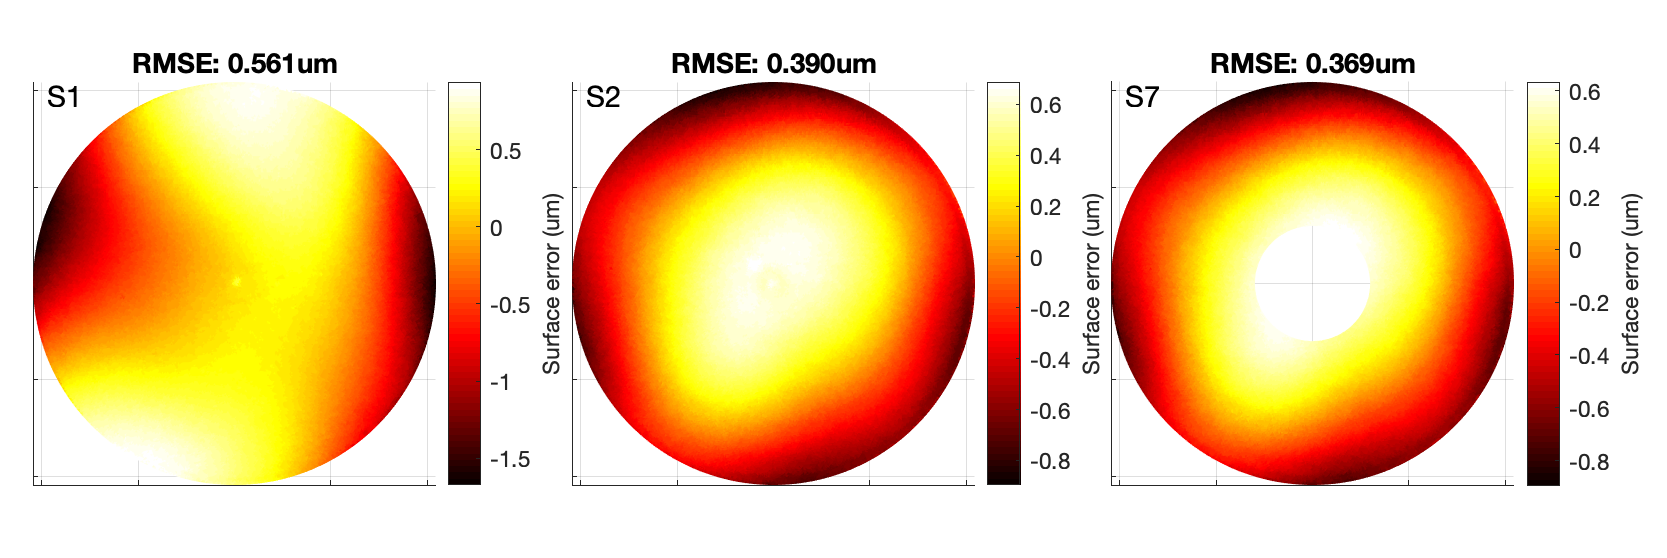
\includegraphics[width=\textwidth]{./pictures/polishing_errorS127.eps}
    \caption{Polishing error surface maps.}
    \label{fig:pol_error_maps}
\end{figure}

Figure~\ref{fig:rho_tradeoff} illustrates the compromise between surface error and magnitude of correction forces. %
%
\begin{figure}[!hbt]
    \vspace{6pt}
    \centering
    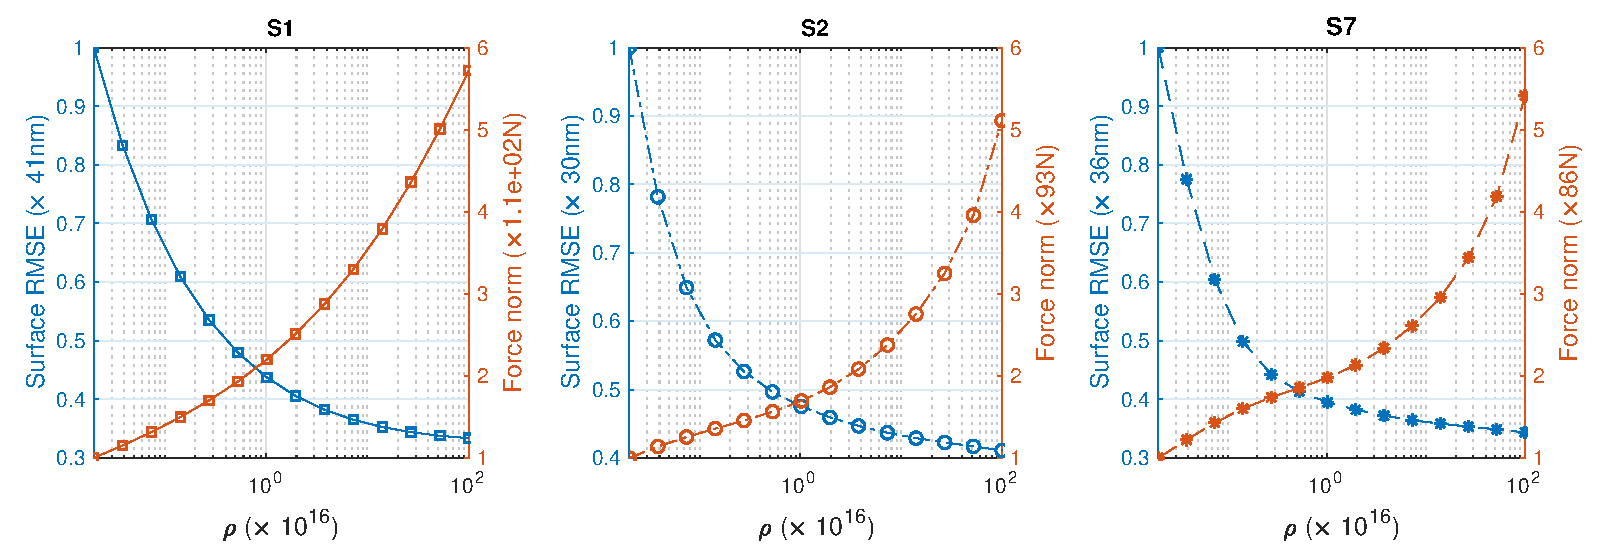
\includegraphics[width=\textwidth]{./pictures/rho_tradeoff_v2.eps}
    \caption{Surface error and magnitude of correction forces trade--off.}
    \label{fig:rho_tradeoff}
\end{figure}
The values are expressed as a factor of the results obtained with the first $\rho$ of the evaluated grid, namely $2\times10^{14}$. From the left to the right, there are three pair of curves: \textsf{S1}, \textsf{S2}, and \textsf{S7}. For the sake of simplicity, we assume $\rho = 10^{16}$ for all segments. Appendix~\ref{sec:alternative_tuning_res} presents further results with alternative trade--off parameter choices.


In the following, we compare the proposed optimization method presented previously with the strategy of compensating the error using the linear subspace formed by the first 27 mirror bending modes. The comparisons are performed in terms of the mirror surface error, the compensation forces magnitude, the local stress induced by those forces and the map of differential forces. The first is quantified through its root mean square (RMS) value of the surface error $s_\epsilon$. Figure~\ref{fig:S1S2S7s_rmse} shows the shapes of the surface error. The forces obtained with the optimization algorithm reduce the surface error obtained after the correction with 27 bending modes by a factor of $20.3$\%, $9.99$\%, and $9.54$\% for segments \textsf{S1}, \textsf{S2}, and \textsf{S7}, respectively.
%------ Surface residual error plots ------%
\begin{figure}[p]
\begin{subfigure}[b]{\textwidth}
\centering
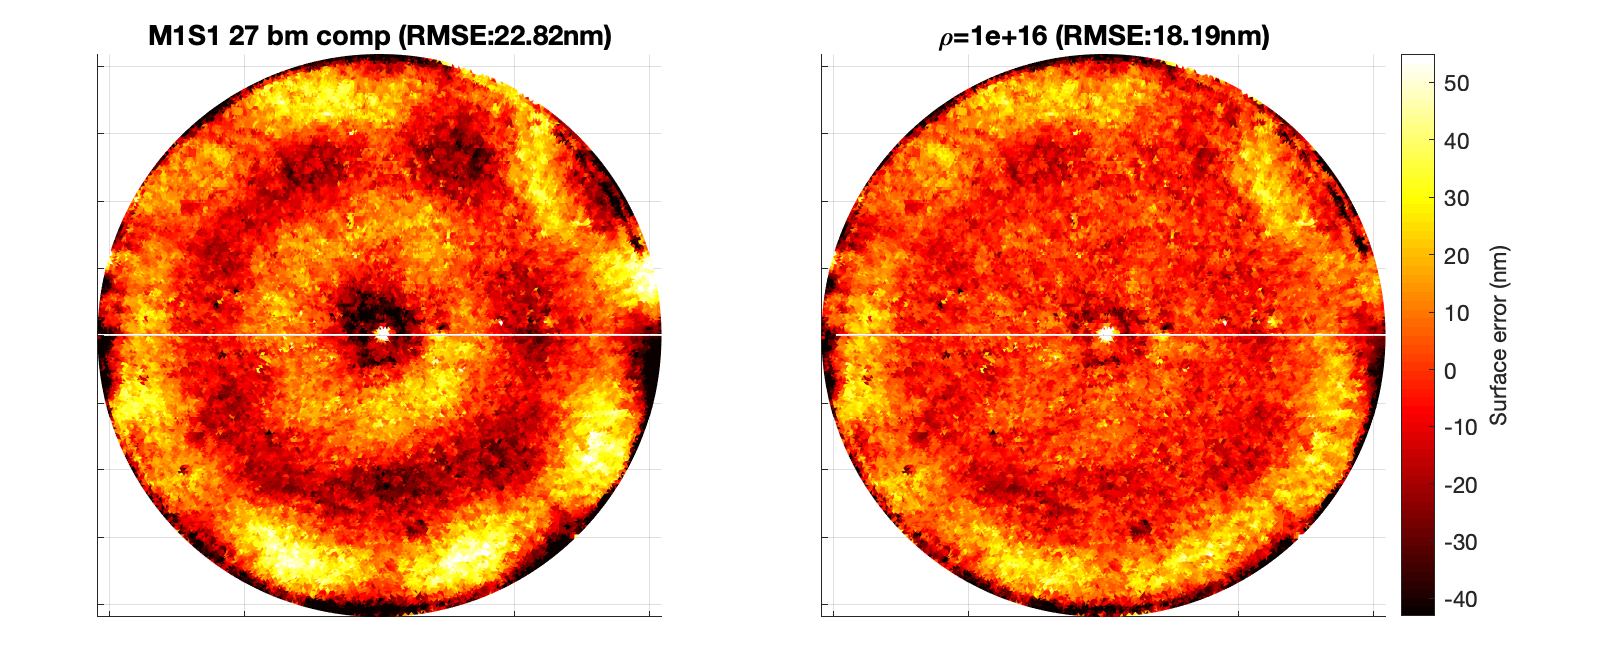
\includegraphics[width=\textwidth]{./pictures/s1_surfaceRMSE.eps}
%\caption{M1S1 residual surface error.}
%\label{fig:S1s_RMSE}
\end{subfigure}
%
\begin{subfigure}[b]{\textwidth}
\centering
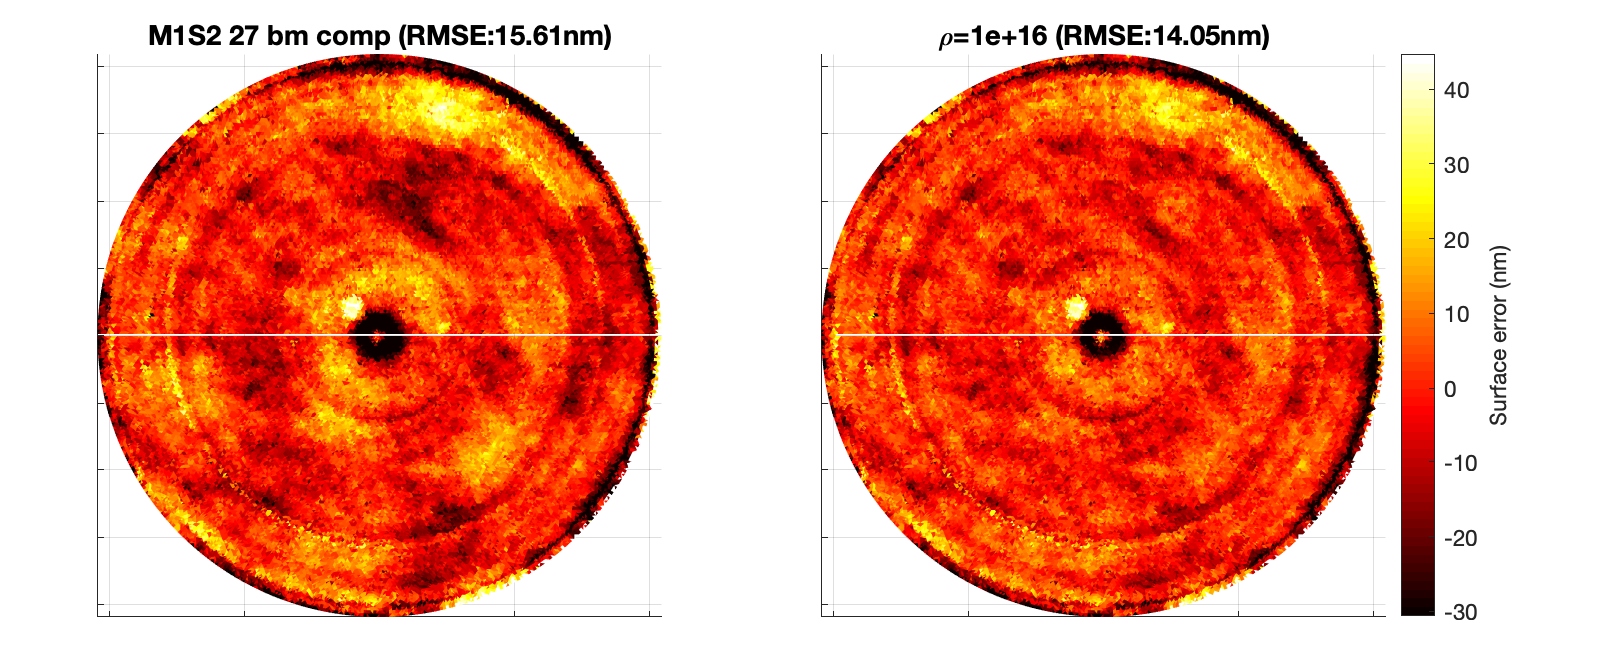
\includegraphics[width=\textwidth]{./pictures/s2_surfaceRMSE.eps}
%\caption{M1S2 residual surface error.}
%\label{fig:S2s_RMSE}
\end{subfigure}
\begin{subfigure}[b]{\textwidth}
\centering
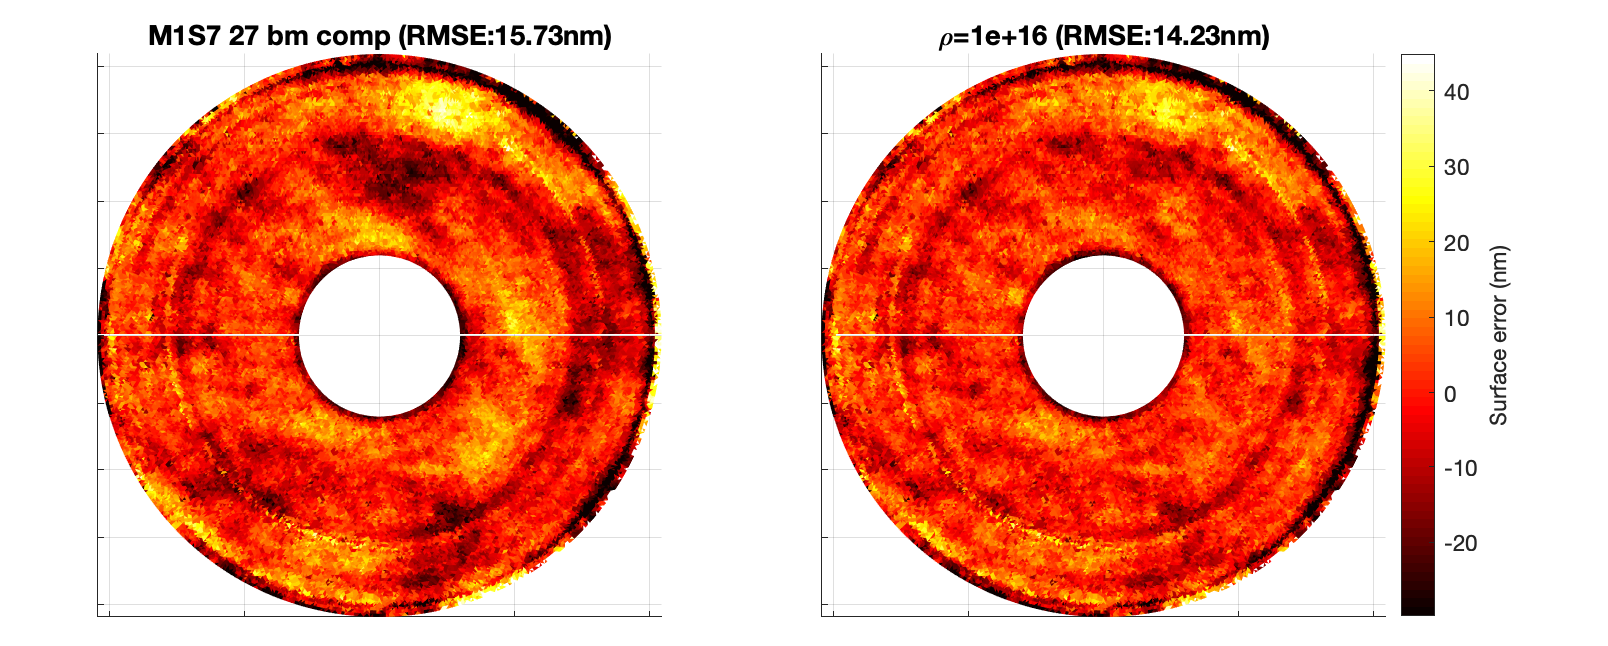
\includegraphics[width=\textwidth]{./pictures/s7_surfaceRMSE.eps}
%\caption{M1S7 residual surface error, based on the S2 fabrication error map.}
%\label{fig:S7s_RMSE}
\end{subfigure}
\caption{\textsf{S1}, \textsf{S2}, and \textsf{S7} residual surface error comparison.}
\label{fig:S1S2S7s_rmse}
\end{figure}


Figures~\ref{fig:s1_forces},~\ref{fig:s2_forces}, and ~\ref{fig:s7_forces} show the polishing error compensation forces for segments \textsf{S1}, \textsf{S2}, and \textsf{S7}, respectively. As a measure of the control effort, it is provided the weighted Euclidean norm of vector $u$, denoted as \[
\|u\|_W = \sqrt{u^T W^T W u} .
\]
%
\begin{figure}[!htb]
\centering
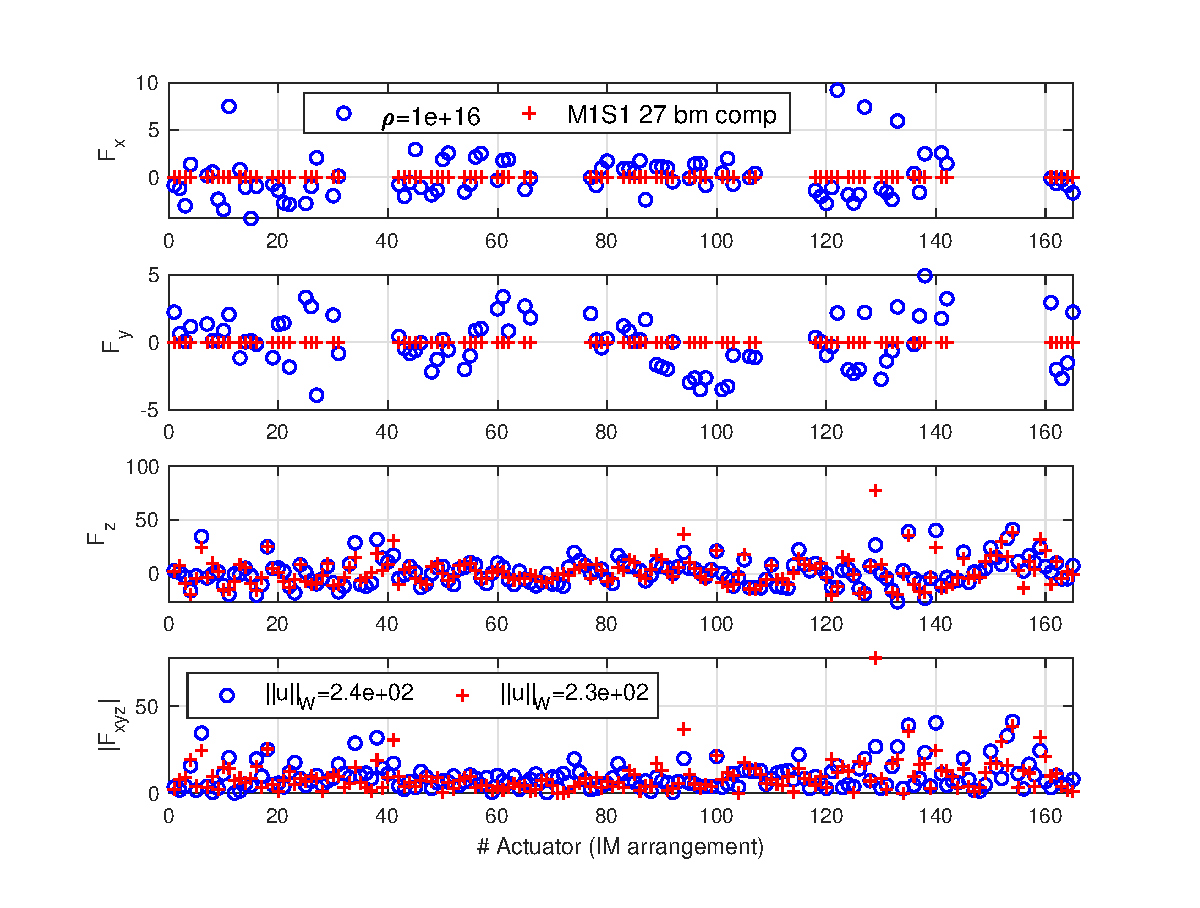
\includegraphics[width=\textwidth]{./pictures/s1_comp_Forces.eps}
\caption{\textsf{S1} fabrication error compensation forces.}
\label{fig:s1_forces}
\end{figure}
\begin{figure}[!htb]
\centering
\includegraphics[width=\textwidth]{./pictures/s2_comp_Forces.eps}
\caption{\textsf{S2} support actuator compensation forces.}
\label{fig:s2_forces}
\end{figure}
\begin{figure}[!htb]
\centering
\includegraphics[width=\textwidth]{./pictures/s7_comp_Forces.eps}
\caption{Center segment compensations forces.}
\label{fig:s7_forces}
\end{figure}
%
% 
There are at least two relevant aspects in the support actuator force comparison. First, besides the axial components %($f_{z_k}$ for $k = \{1, 2, \ldots, n_a \}$)
 as the forces required to compensate for the deformations projected onto the first $27$ bending modes, the proposed algorithm uses lateral %($f_{x_k}$)
  and cross--lateral %($f_{y_k}$)
  forces. Second, though the methods lead to similar force norms for $\rho=10^{16}$ (Table~\ref{tab:Wnorm_u}), the quadratic cost function \eqref{eq:J} prevents high--force values, indicating that the compensation is better distributed between the support actuators. See, for instance, the comparison for the axial forces of actuator \#129 in segment \textsf{S1} (Figure~\ref{fig:s1_forces}).
\begin{table}[!htb]
\centering
\caption{Weighted norm of the polishing error compensation forces.}
\label{tab:Wnorm_u}
\begin{tabular}{l|ccc}
 & \textsf{S1} & \textsf{S2} & \textsf{S7}\\
 \hline
27 BM compensation & \SI{230}{\newton} & \SI{160}{\newton} & \SI{180}{\newton}\\
Optimization algorithm & \SI{240}{\newton} & \SI{160}{\newton} & \SI{170}{\newton}
\end{tabular}
\end{table}

One can also notice that magnitudes of the forces required to compensate for the \textsf{S1} surface error are higher, than for the other segments. In fact, the \textsf{S1} polishing error is the highest: \SI{0.56}{\micron} RMSE against \SI{0.39}{\micron} and \SI{0.369}{\micron}, for segments \textsf{S2} and \textsf{S7}, respectively.


The most significant surface error improvement (with respect to the correction considering the first 27 bending modes) and highest force norm observed for \textsf{S1} may suggest a more aggressive tuning for that particular segment, compared to the others. However, the subsequent analysis indicates that in order to achieve further mirror shape improvement, it can be more compelling to increase the value of the parameter $\rho$ for \textsf{S1} and \textsf{S7}, than for \textsf{S2}.

 Figures~\ref{fig:s1_ng_sigma},~\ref{fig:s2_ng_sigma}, and ~\ref{fig:s7_ng_sigma} depict the maximum neighborhood differential force (at the top) and the local stress (at the bottom) induced by the compensation forces on segments \textsf{S1}, \textsf{S2}, and \textsf{S7}, respectively. %
\begin{figure}[!htb]
\centering
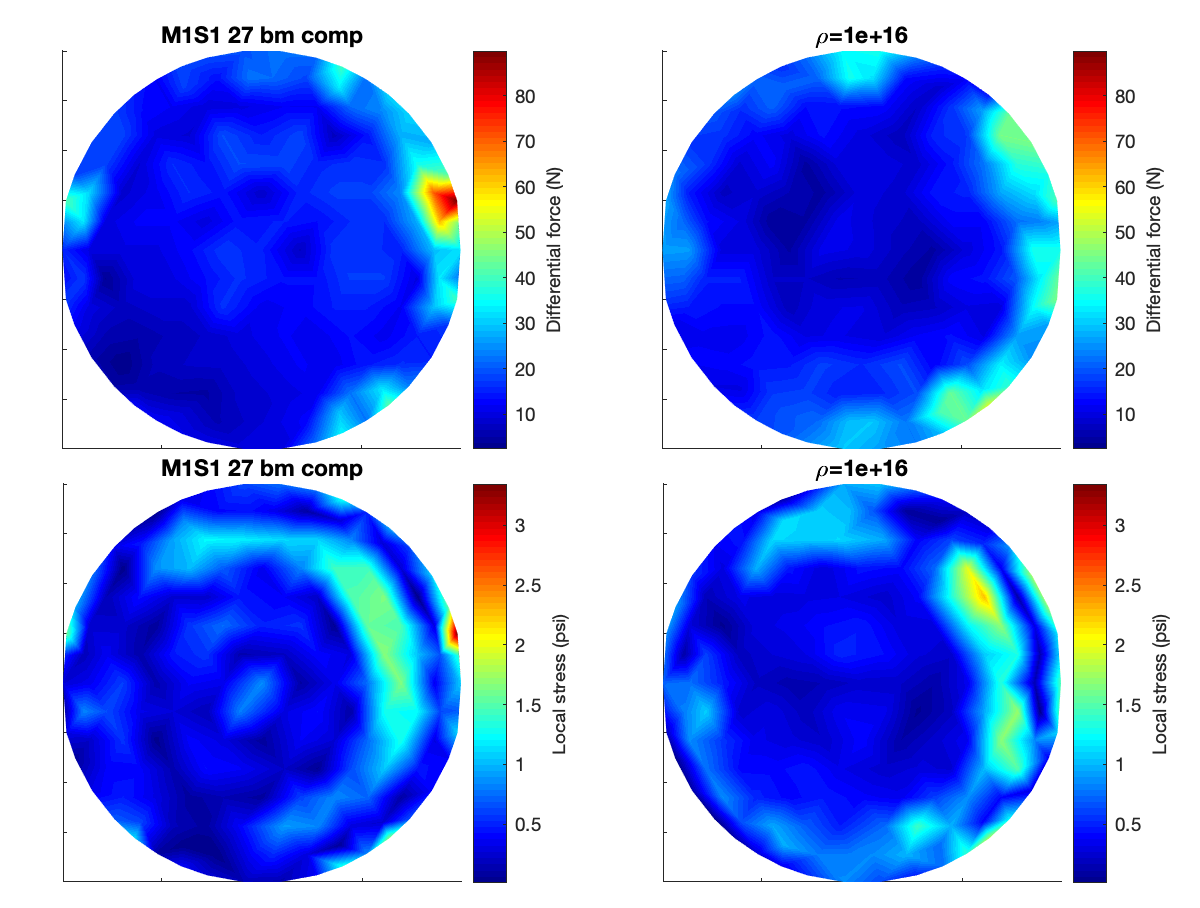
\includegraphics[width=\textwidth]{./pictures/s1_NG_sigma.eps}
\caption{\textsf{S1} maximum neighborhood force gradient and local stress.}
\label{fig:s1_ng_sigma}
\end{figure}
\begin{figure}[!htb]
\centering
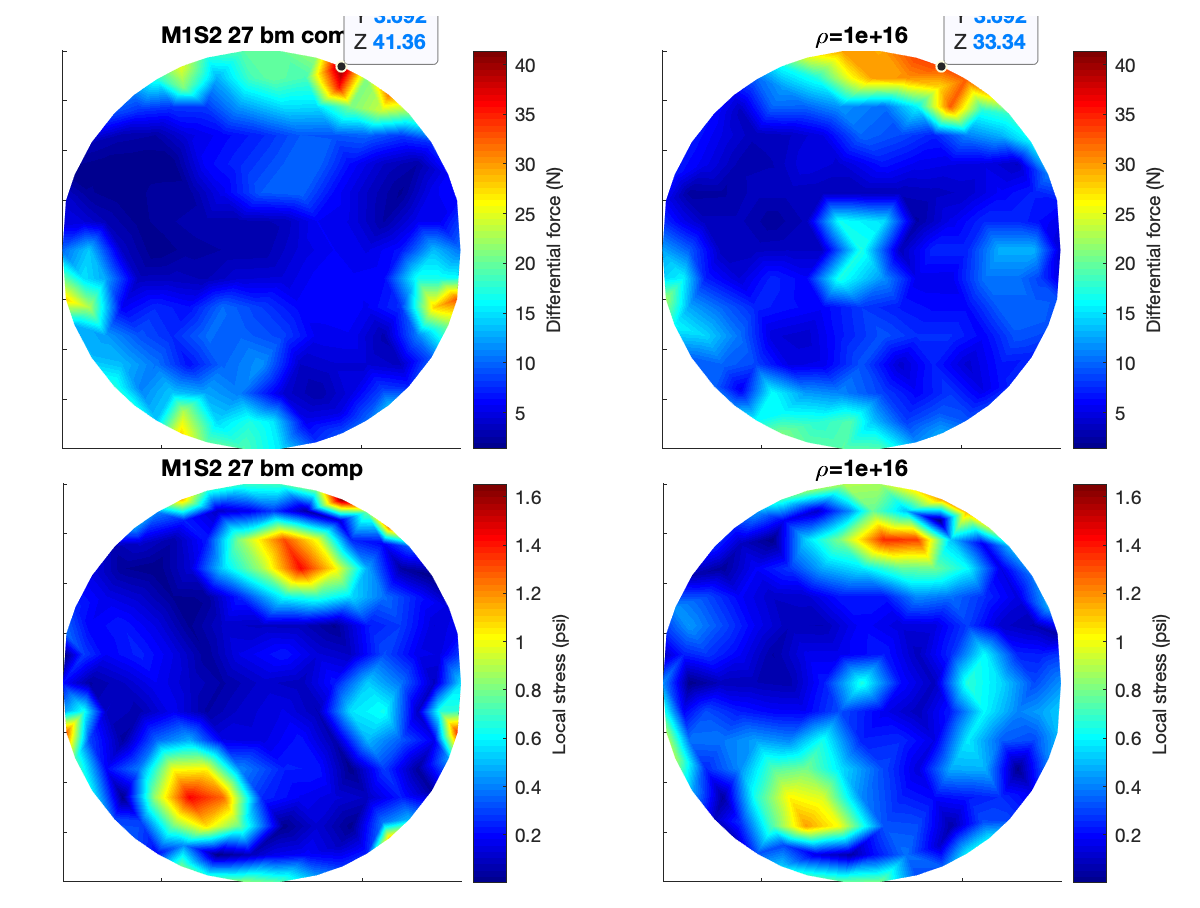
\includegraphics[width=\textwidth]{./pictures/s2_NG_sigma.eps}
\caption{Maximum neighborhood differential force and local stress on \textsf{S2}.}
\label{fig:s2_ng_sigma}
\end{figure}
\begin{figure}[!htb]
\centering
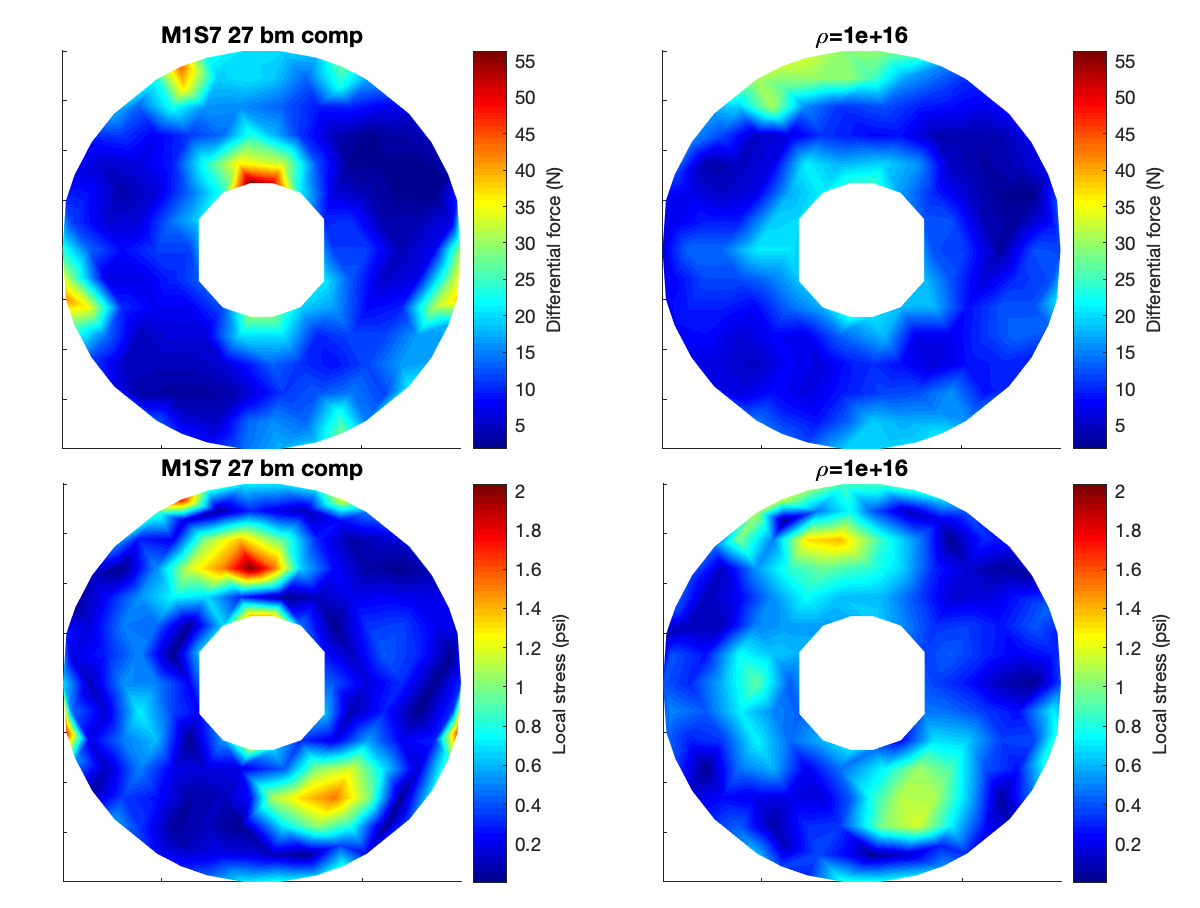
\includegraphics[width=\textwidth]{./pictures/s7_NG_sigma.eps}
\caption{\textsf{S7} maximum neighborhood differential force and local stress.}
\label{fig:s7_ng_sigma}
\end{figure}
The differential force can be seen as an indication of mirror glass tension\todo{Do you agree with that statement?}. Therefore, we compute the maximum differential resultant force with respect to the  neighborhood of each actuator. The approximate local stress $\sigma$ produced by the $k$th actuator is given by \cite[Subsection~4.1.6]{gmtM1req}
\[\sigma_k = \sqrt{w_\text{ax}^2 f_{z_k}^2 + w_\text{lat}^2\left(f_{x_k}^2 + f_{y_k}^2\right)}, \]
%
where the axial and lateral weights lateral force weights are
\begin{align*}
    w_\text{ax} & = \left\{
    \begin{array}{ll}
         0.0852\text{psi/N} & \text{ , for} f_{z_k} \geq 0\text{ (axial push)}\\
         0.0429\text{psi/N} & \text{ , for} f_{z_k} < 0\text{ (axial pull)}
    \end{array}
    \right. \\
    w_\text{lat} & = 0.0782\text{psi/N}.
\end{align*}

Figure~\ref{fig:s1_ng_sigma} shows that the baseline correction leads to a gradient peak of almost \SI{90}{\newton} at the edge on the right--side of segment \textsf{S1}, while the forces obtained from \ref{eq:alternative_u} never exceed \SI{53}{\newton}. The local stress comparison confirms that the proposed method distributes better the compensation forces. The highest value is reduced from \SI{3.34}{psi} to \SI{2.27}{psi} ($32$\%). The results for segments \textsf{S2} and \textsf{S7} follow the same trend. Nevertheless, the benefits of the proposed approach in terms of differential force and local stress obtained for \textsf{S2} are more modest (\ref{fig:s2_ng_sigma}). Hence, there is less margin to improve the surface error by increasing the parameter $\rho$. %


In summary, the previous results confirm that besides achieving a significant surface error mitigation, the proposed optimization method reduces the local stress and the differential force over the mirror, particularly concerning \textsf{S1} and \textsf{S7} --- in those cases, there is considerable room for further improvement. The complementary simulation results reported in Appendix~\ref{sec:alternative_tuning_res} illustrate those points.


At last, we evaluate the impact of the compensated surface shapes on the image quality in the telescope exit pupil. It is fair to expect that that the same quality will carry through the fabrication shapes of the upcoming mirrors. So, as in~\cite{GMT_DOC_04637}, we assume the \textsf{S2} polishing error map for segments \textsf{S2}--\textsf{S7}.


Using the algorithm of Section~\ref{sec:opt_method}, the resulting Normalized Point Source Sensitivity (PSSN\footnote{
For the Natural Seeing (NS) operating mode, in which adaptive optics corrections are not performed, the closer to 1, the better is the image. One is referred to \cite[Section~3]{GMT_DOC_04680} for a formal definition of the PSSN.
}) is $0.9680$\todo{Update PSSN!} 
at \SI{0.5}{\micron}, which is a relevant improvement compared to the $0.9563$ obtained  after the first 27 bending modes are filtered from the polishing error map of the primary mirror segments.









\section{Concluding Remarks}
\label{sec:conclusions}


An optimization method is developed to compute forces to correct surface fabrication errors through open-loop (offset) commands. The simulation results are promising. Besides improving the optical surface shape substantially, compared to the baseline compensation that has been considered so far, there are indications that the obtained compensation forces induce less tension on the mirror glass.

This study assumes that fabrication errors and gravity print-through are addressed separately. However,  it can be even more advantageous to incorporate fabrication errors in a surface deformation model induced by gravity and then, to handle the computation of the M1 support actuator forces in a unified approach.


\printbibliography

\clearpage \newpage

\appendix


\section{Complementary simulations results}
\label{sec:alternative_tuning_res}

Motivated by the differential force and local stress results, we assess forces obtained with the method described in Section~\ref{sec:opt_method} considering $\rho$ equal to $4\times10^{16}$ and $3\times10^{16}$, for the segments \textsf{S1} (Figure~\ref{fig:s1_altrho_results}) and \textsf{S7} (Figure~\ref{fig:s7_altrho_results}), respectively.  We also evaluated \textsf{S2} assuming $\rho=2\times 10^{16}$. This more conservative increase on the parameter $\rho$ (recall that in Section~\ref{sec:simulations} one considers $\rho=10^{16}$) is due to the modest margin of improvement observed in Figure~\ref{fig:s2_ng_sigma}. Those parameter values were chosen to improve further the mirror shapes reported in Figure~\ref{fig:S1S2S7s_rmse}. At the same time, the new parameter values are expected achieve lower differential forces and local stress peaks than the baseline compensation forces. %
Table~\ref{tab:altrho_results} summarizes the results obtained. To ease comparisons, in the parenthesis, we report the results provided by the compensation based on the first 27 bending modes. 
\begin{table}[!htb]
\centering
\caption{Results summary with the proposed approach assuming an alternative tuning.}
\label{tab:altrho_results}
\begin{tabular}{l|ccc}
 & Surface RMSE & Max differential force & Max local stress \\
 \hline
\textsf{S1} & \SI{15.79}{nm} (\SI{22.82}{nm}) & \SI{80.8}{\newton} (\SI{89.8}{\newton}) & \SI{2.72}{psi} (\SI{3.34}{psi})\\
\textsf{S2} & \SI{13.55}{nm} (\SI{15.61}{nm}) & \color{red}{\SI{41.9}{\newton}} (\SI{41.4}{\newton}) & \SI{1.4}{psi} (\SI{1.46}{psi})\\
\textsf{S7} & \SI{13.51}{nm} (\SI{15.73}{nm}) & \SI{46.7}{\newton} (\SI{56.3}{\newton}) & \SI{1.43}{psi} (\SI{2.03}{psi})
\end{tabular}
\end{table}

The new tuning improves the \textsf{S1}, \textsf{S2}, and \textsf{S7} residual errors obtained with the correction based on the first $27$ bending modes by a factor of $30.8$\%, $13.2$\%, and $14.1$\%, respectively. The proposed algorithm alternative tuning reduces the maximum differential force and local stress peaks of the baseline correction for segments \textsf{S1} and \textsf{S7}. In contrast, even the more conservative \textsf{S2} retuning leads to similar local stress peak values and worsens the differential force profile (see Figure~\ref{fig:s2_altrho_results}).

\todo[inline]{* * * Include PSSN info * * *}

\begin{figure}[!p]
\centering
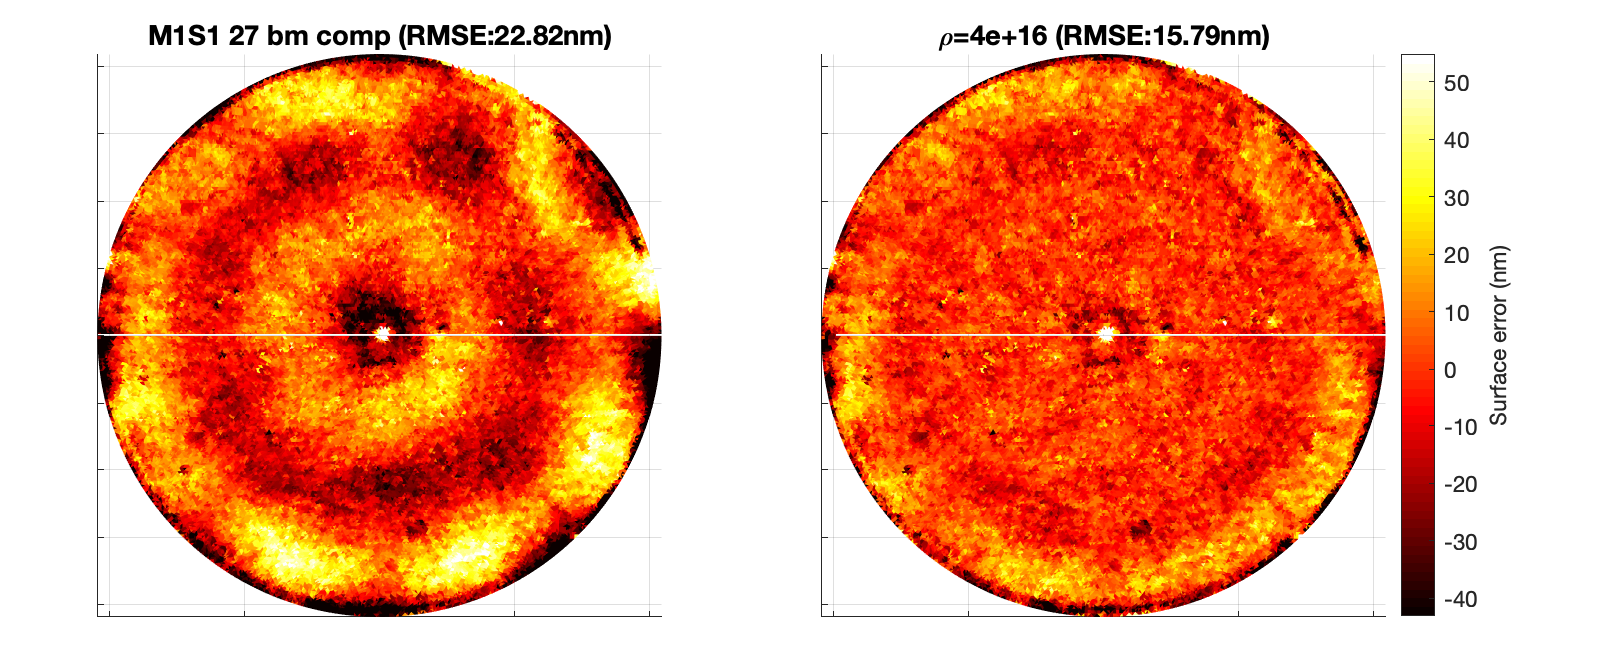
\includegraphics[width=\textwidth]{./pictures/s1_surfaceRMSE_rho4e16.eps}
\vfill
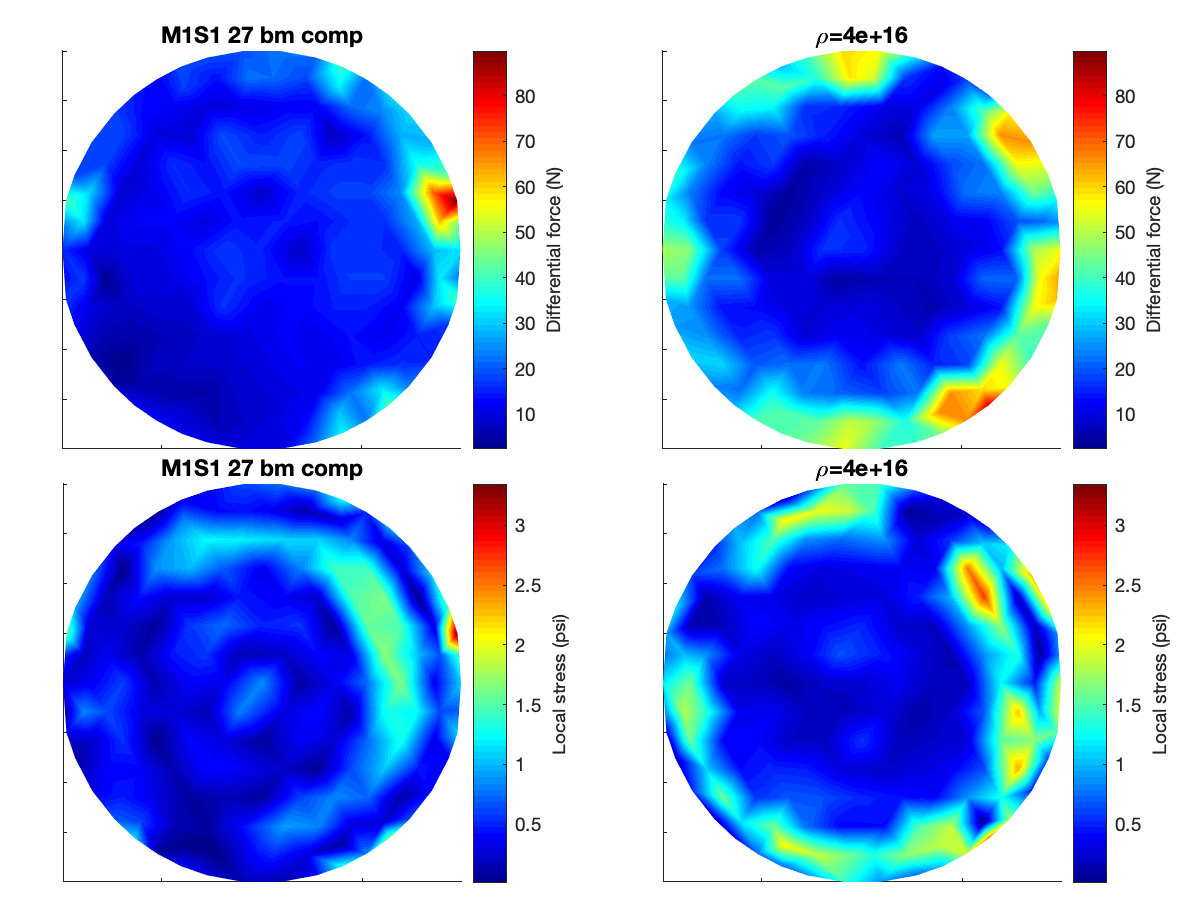
\includegraphics[width=\textwidth]{./pictures/s1_NG_sigma_rho4e16.eps}
\caption{\textsf{S1} results assuming $\rho=4\times10^{16}$.}
\label{fig:s1_altrho_results}
\end{figure}



\begin{figure}[!p]
\centering
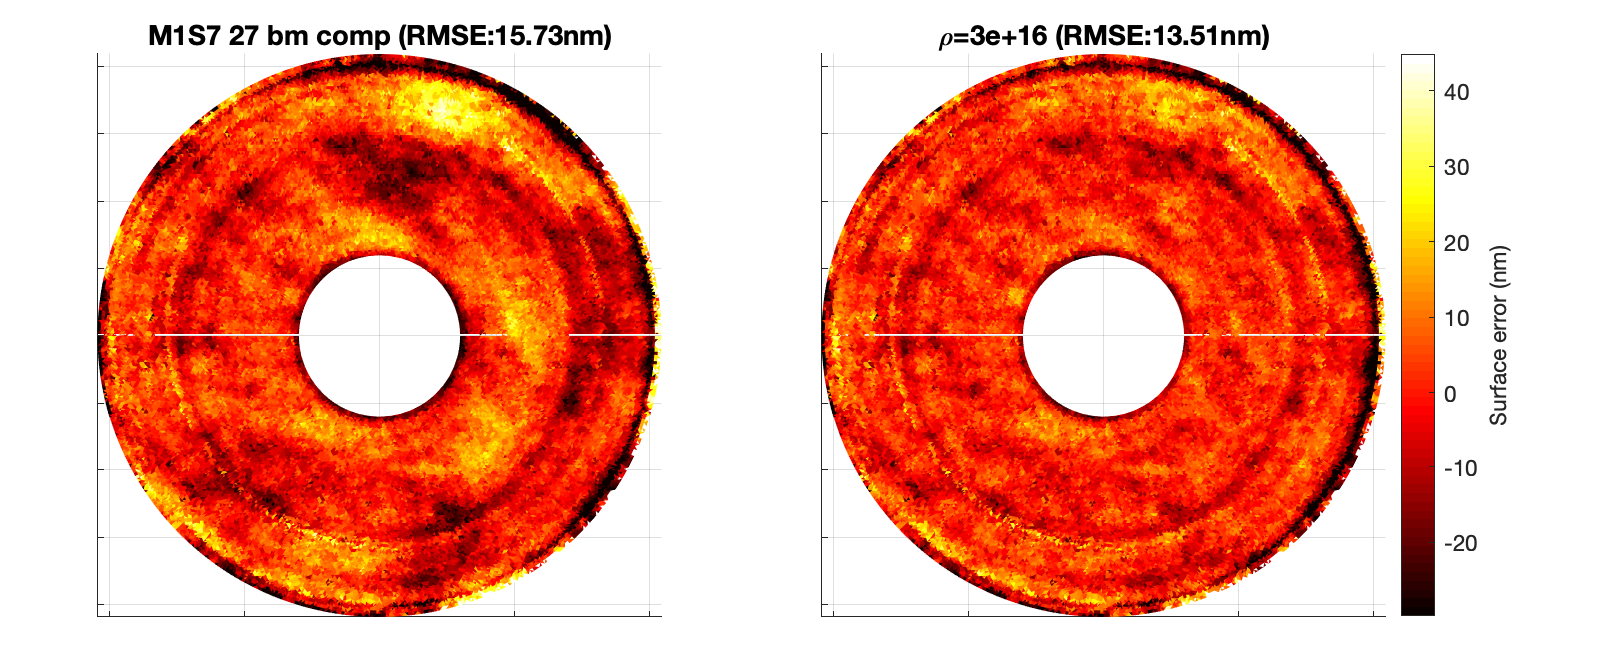
\includegraphics[width=\textwidth]{./pictures/s7_surfaceRMSE_rho3e16.eps}
\vfill
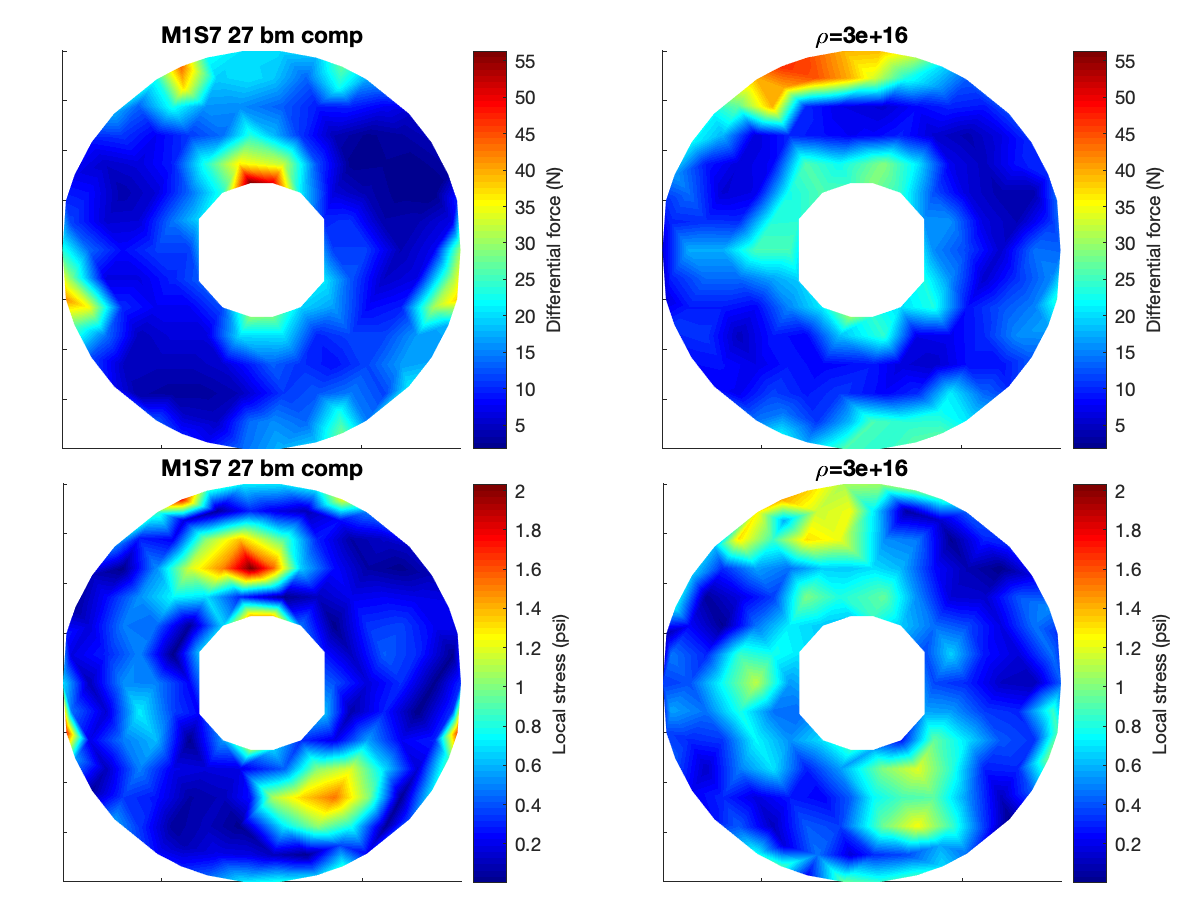
\includegraphics[width=\textwidth]{./pictures/s7_NG_sigma_rho3e16.eps}
\caption[\textsf{S7} results assuming a more aggressive surface correction]{\textsf{S7} results assuming a more aggressive surface correction ($\rho=3\times10^{16}$).}
\label{fig:s7_altrho_results}
\end{figure}



\begin{figure}[!p]
\centering
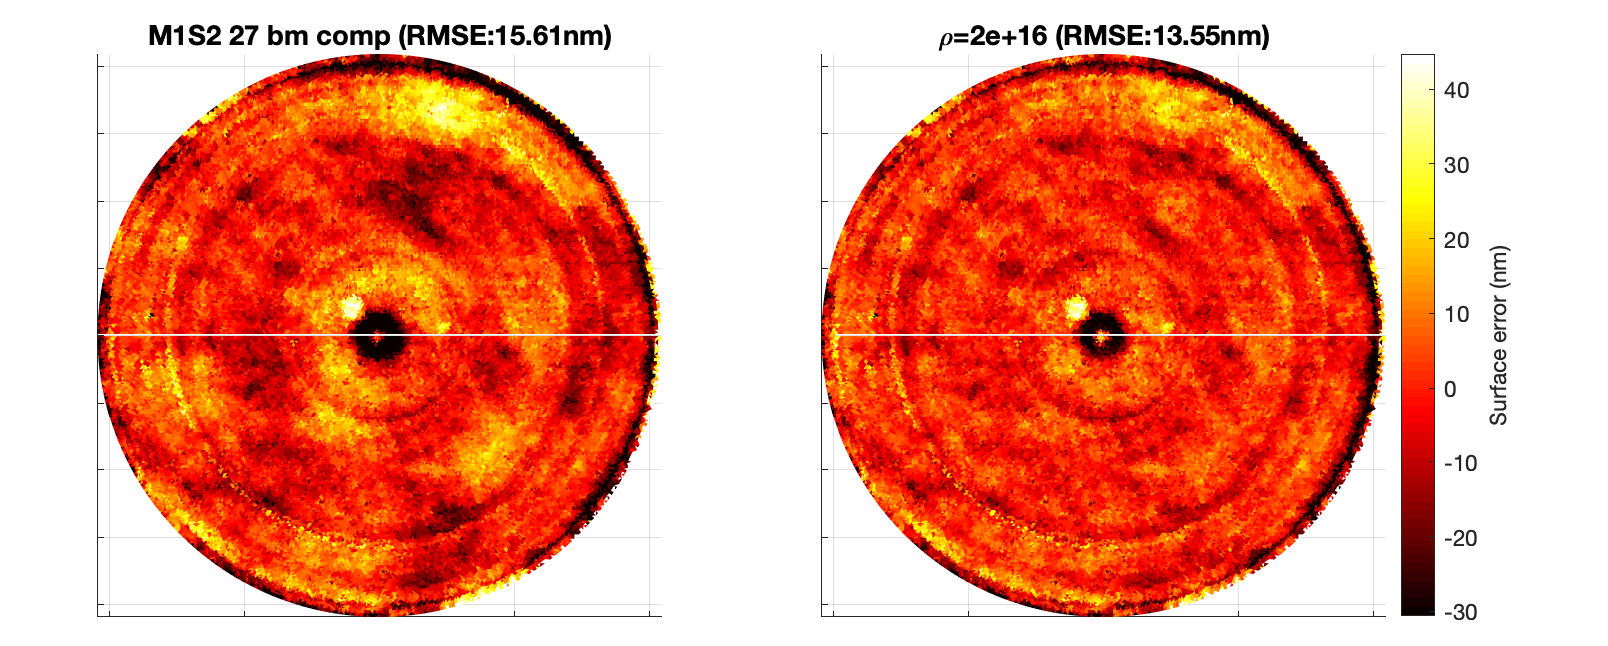
\includegraphics[width=\textwidth]{./pictures/s2_surfaceRMSE_rho2e16.eps}
\vfill
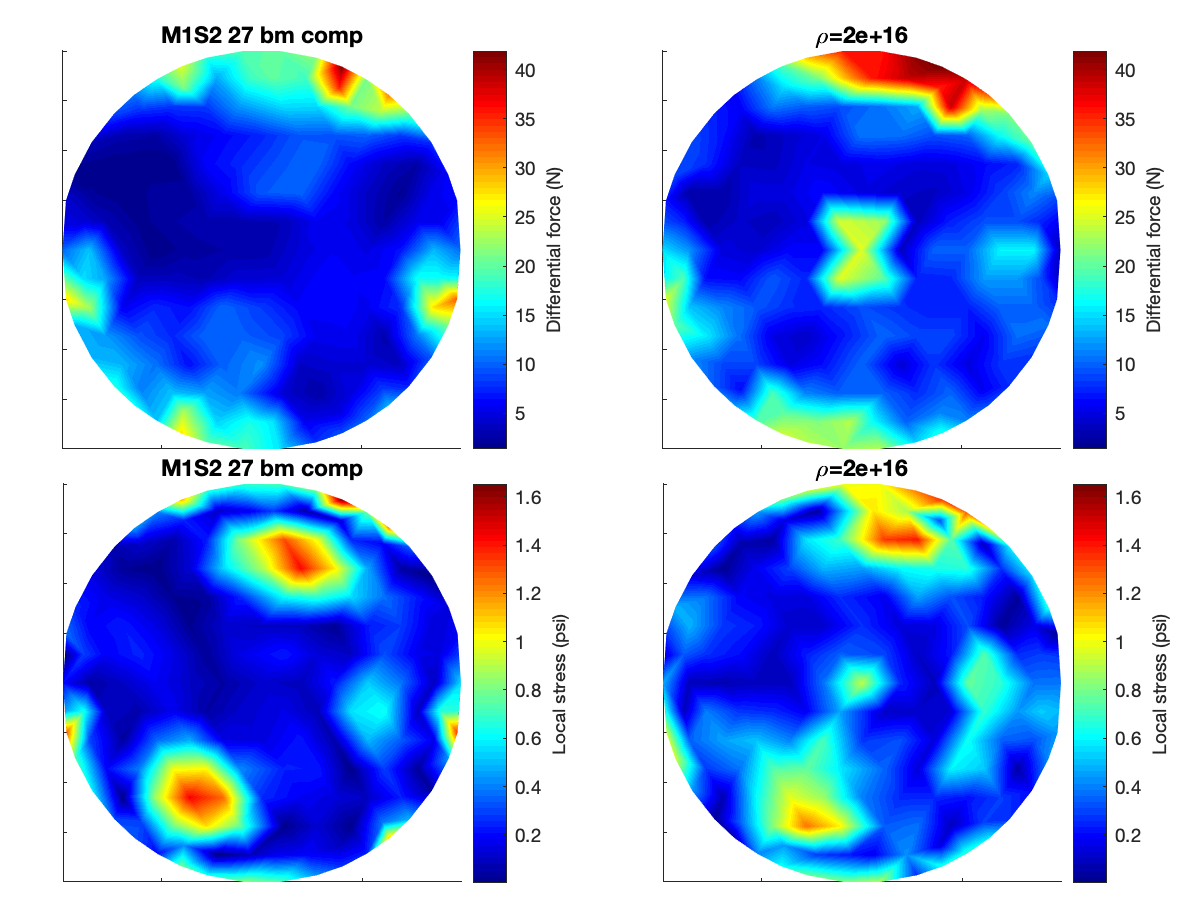
\includegraphics[width=\textwidth]{./pictures/s2_NG_sigma_rho2e16.eps}
\caption{\textsf{S2} results assuming an alternative optimization algorithm tuning.}
\label{fig:s2_altrho_results}
\end{figure}



\clearpage \newpage
\section{Optimization Problem Solution}
\label{sec:OPT_sol}

To solve \eqref{eq:LSOproblem}, subject to $\tau = \Upsilon u$, define the Lagragian function
\[
\mathcal{L}(u,\lambda) = \frac{\rho}{2}\left( s_{\text{p}} + A_f M_r^\dagger u \right)^T\left( s_{\text{p}} + A_f M_r^\dagger u \right) + \frac{1}{2} \left(Wu\right)^T\left(Wu\right) - \lambda^T \left(\tau - \Upsilon u\right) ,
\]
where $\lambda \in \mathbb{R}^6$ is the vector of Lagrange multipliers.% introduced to handle the constraint.

The optimal solution $u^\ast$ satisfies
%
\begin{align*}
    % \label{eq:dLagrangian1}
    \frac{\mathcal{L}}{\delta u} & = 
    \rho \Lambda^T s_{\text{p}} + \left(\rho\Lambda^T\Lambda + W^TW\right) u 
    + \lambda^T \Upsilon = 0 \\
    % \label{eq:dLagrangian2}
    \frac{\mathcal{L}}{\delta \lambda} & = \tau - \Upsilon u = 0 ,
\end{align*}
where $\Lambda = A_f M_r^\dagger$.

Those optimality conditions can be written as a linear system
\[
\begin{bmatrix}
\rho \Lambda^T\Lambda + W^TW & \Upsilon^T \\ \Upsilon & 0_{6 \times 6}
\end{bmatrix}
\begin{bmatrix}
u \\ \lambda
\end{bmatrix}
=
\begin{bmatrix}
- \rho \Lambda^T s_{\text{p}} \\ \tau
\end{bmatrix} ,
\]
whose solution is
\begin{equation}
\label{eq:OPT_lsys}
\begin{bmatrix}
u \\ \lambda
\end{bmatrix}
=
\begin{bmatrix}
\rho \Lambda^T\Lambda + W^TW & \Upsilon^T \\ \Upsilon & 0_{6 \times 6}
\end{bmatrix}^{-1}
\begin{bmatrix}
- \rho \Lambda^T s_{\text{p}} \\ \tau
\end{bmatrix}.
\end{equation}

From \eqref{eq:OPT_lsys}, the solution for $u$ can be written as
\[
u = 
\begin{bmatrix}
I_{n_u} & \mathbf{0}_{n_u \times 6}
\end{bmatrix}
\begin{bmatrix}
\rho \Lambda^T\Lambda + W^TW & \Upsilon^T \\ \Upsilon & \mathbf{0}_{6 \times 6}
\end{bmatrix}^{-1} \begin{bmatrix}
- \rho \Lambda^T s_{\text{p}} \\ \tau
\end{bmatrix},
\]
where $I_{n_u}$ is an $n_u$--dimensional identity matrix and $\mathbf{0}_{n_1 \times n_2}$ represents $n_1 \times n_2$--dimensional matrices filled with zeros.

\end{document}


